%%%%%%%%%%%%%%%%%%%%%%%%%%%%%%%%%%%%%%%%%%%%%%%%%%%%%%%%%%%%%%%%%%%%%%%%%%%%%%%%
% event_selection.tex: 
%%%%%%%%%%%%%%%%%%%%%%%%%%%%%%%%%%%%%%%%%%%%%%%%%%%%%%%%%%%%%%%%%%%%%%%%%%%%%%%%
\chapter{Event Selection}
\label{sec:event_selection_chapter}
%%%%%%%%%%%%%%%%%%%%%%%%%%%%%%%%%%%%%%%%%%%%%%%%%%%%%%%%%%%%%%%%%%%%%%%%%%%%%%%%

LRS models presented earlier predict the existence of a \WR boson and heavy neutrinos \nul, and that their 
production and decay yields events with two high energy jets and two high energy charged leptons.  Using 
the 2.6 fb$^{-1}$ \cite{lumi} of collision data recorded by CMS from September through November 2015, evidence of 
\WR and \nul production was searched for in events with $\ell\ell jj$ ($\ell = e,\mu$) final states.  
Events were selected using lepton and jet selections developed from features of expected ST backgrounds 
and $\WR \rightarrow \ell\nul \rightarrow \ell\ell jj$ decays.


\section{\WR and \nul Signal Features}
\label{sec:signalFeatures}
Lepton and jet selections were driven by several model-independent features of \WR and \nul decays.  The \WR mass 
(\mWR) was expected to be large, 2 $\TeV$ or more, relative to the center-of-mass collision energy of 13 $\TeV$, 
so \WR bosons would have been produced with low momentum.  Therefore, the charged lepton and jet decay 
products, on average, were distributed uniformly in $\phi$, and concentrated in the region $|\eta| < 2.4$, 
as shown in Figures \ref{fig:wrLeptonEtas} and \ref{fig:wrJetEtas}.  Furthermore, the large expected 
\mWR yielded leptons and jets with several hundred $\GeV$ or more of $\pt$, as shown in 
Figures \ref{fig:wrLeptonPts} and \ref{fig:wrJetPts}.  The $\eta$ and $\pt$ distributions of final state 
particles, and the large expected \mWR motivated the following selections on charged leptons and jets in 
every event:

\begin{itemize}
	\item Two leptons were reconstructed with $\pt$ or $\Et > 53$ $\GeV$, and one had $\pt$ or $\Et > 60$ $\GeV$.
	\item Two jets were reconstructed with $\pt > 40$ $\GeV$.
	\item Both leptons and jets were reconstructed with $|\eta| < 2.4$.
	\item The invariant mass $\Mlljj$ of the selected leptons and jets exceeded $\Mlljj > 600$ $\GeV$.
\end{itemize}

The large predicted mass difference between the charged lepton $\ell$ and heavy neutrino \nul yielded 
additional distinguishing features of the signal.  To conserve momentum in the $\WR \rightarrow \ell \nul$ 
decay, the charged lepton $\ell$ recoiled against the heavier neutrino \nul.  Then the \nul decayed to a 
second charged lepton and two jets that recoiled against the first charged lepton.  Thus the lepton pair, 
on average, had a large dilepton mass $\Mll$ (Figure \ref{fig:wrSigMll}), and the first charged 
lepton\footnote{produced with the \nul} was often well separated in $(\eta, \phi)$ from the \nul decay 
products (Figure \ref{fig:wrLeadLeptJetSeparation}).  The large expected neutrino mass \mnul, hundreds of 
$\GeV$ or more, needed to predict low ST neutrino masses usually resulted in large $(\eta, \phi)$ separations 
between \nul decay products, as shown in Figure \ref{fig:wrSubleadLeptJetSeparation}.  The $(\eta, \phi)$ 
separation between charged leptons and jets, and the recoil of one charged lepton against the \nul 
decay products motivated additional event selections:

\begin{itemize}
	\item Each selected lepton was separated from both selected jets by $\Delta R > 0.4$.
	\item The dilepton mass $\Mll$ of the two selected leptons exceeded $\Mll > 200$ $\GeV$.
\end{itemize}


\begin{figure}[btp]
	\centering
	\subfigure{
		
\includegraphics[width=0.65\textwidth]{figures/missingImage.png}
	}
	\subfigure{
		
\includegraphics[width=0.65\textwidth]{figures/missingImage.png}
	}
	\label{fig:wrLeptonEtas}
	\caption{The $\eta$ distribution of the leading (sub-leading) reconstructed muon is shown on the left (right) for 
		$\WR \rightarrow \mu\mu jj$ events with $\mWR = 2.0 \TeV$ and $\mnul = 1.0 \TeV$.  The electron 
	distributions are identical, except for the ECAL barrel-endcap gap where electrons are not reconstructed.}
\end{figure}

\begin{figure}[btp]
	\centering
	\subfigure{
		
\includegraphics[width=0.65\textwidth]{figures/missingImage.png}
	}
	\subfigure{
		
\includegraphics[width=0.65\textwidth]{figures/missingImage.png}
	}
	\label{fig:wrJetEtas}
	\caption{The $\eta$ distribution of the leading (sub-leading) reconstructed jet is shown on the left (right) for 
		$\WR \rightarrow \mu\mu jj$ events with $\mWR = 2.0 \TeV$ and $\mnul = 1.0 \TeV$.}
\end{figure}

\begin{figure}[btp]
	\centering
	\subfigure{
		
\includegraphics[width=0.65\textwidth]{figures/missingImage.png}
	}
	\subfigure{
		
\includegraphics[width=0.65\textwidth]{figures/missingImage.png}
	}
	\label{fig:wrLeptonPts}
	\caption{The $\pt$ distribution of the leading (sub-leading) reconstructed muon is shown on the left (right) for 
		$\WR \rightarrow \mu\mu jj$ events with $\mWR = 2.0 \TeV$ and $\mnul = 1.0 \TeV$.}
\end{figure}

\begin{figure}[btp]
	\centering
	\subfigure{
		
\includegraphics[width=0.65\textwidth]{figures/missingImage.png}
	}
	\subfigure{
		
\includegraphics[width=0.65\textwidth]{figures/missingImage.png}
	}
	\label{fig:wrJetPts}
	\caption{The $\pt$ distribution of the leading (sub-leading) reconstructed jet is shown on the left (right) for 
		$\WR \rightarrow \mu\mu jj$ events with $\mWR = 2.0 \TeV$ and $\mnul = 1.0 \TeV$.}
\end{figure}

\begin{figure}[btp]
	\centering
	
\includegraphics[width=0.65\textwidth]{figures/missingImage.png}
	\label{fig:wrSigMll}
	\caption{The distribution of the dilepton mass $\Mll$ for $\WR \rightarrow \mu\mu jj$ events with 
	$\mWR = 2.0 \TeV$ and $\mnul = 1.0 \TeV$.}
\end{figure}

\begin{figure}[btp]
	\centering
	\subfigure{
		
\includegraphics[width=0.65\textwidth]{figures/missingImage.png}
	}
	\subfigure{
		
\includegraphics[width=0.65\textwidth]{figures/missingImage.png}
	}
	\label{fig:wrLeadLeptJetSeparation}
	\caption{The $\Delta R(\ell,j)$ separation between the leading reconstructed muon and leading (sub-leading) reconstructed jet 
		is shown on the left (right) for $\WR \rightarrow \mu\mu jj$ events with $\mWR = 2.0 \TeV$ and $\mnul = 1.0 \TeV$.}
\end{figure}

\begin{figure}[btp]
	\centering
	\subfigure{
		
\includegraphics[width=0.65\textwidth]{figures/missingImage.png}
	}
	\subfigure{
		
\includegraphics[width=0.65\textwidth]{figures/missingImage.png}
	}
	\label{fig:wrSubleadLeptJetSeparation}
	\caption{The $\Delta R(\ell,j)$ separation between the sub-leading reconstructed muon and leading (sub-leading) reconstructed jet 
		is shown on the left (right) for $\WR \rightarrow \mu\mu jj$ events with $\mWR = 2.0 \TeV$ and $\mnul = 1.0 \TeV$.}
\end{figure}


\section{Online Event Selection}
\label{sec:triggers}
Evidence of \WR and \nul production was searched for in events selected by lepton triggers.  Events 
used in the $ee$-channel search were selected with a double electron HLT algorithm, and events used 
in the $\mu\mu$-channel search were selected with a single muon HLT algorithm.

In the $ee$-channel search events were selected by Level-1 triggers that required one ECAL supercluster 
(SC) with $\Et > 40 \GeV$, or a pair of non-overlapping SCs - one with $\Et > 22$ $\GeV$, the other with 
$\Et > 10$ $\GeV$.  Events that passed the L1 selection were reconstructed if they passed the 
following double electron HLT selections:

\begin{itemize}
	\item Two non-overlapping SCs were detected with $\Et > 33$ $\GeV$.
	\item For each SC:
	\begin{itemize}
		\item The ratio of hadronic energy in the HCAL tower behind the SC to the SC energy was $< 0.15$ in the barrel, and $< 0.1$ in the endcap.
		\item Ninety percent of the SC energy was measured in an $(\eta, \phi)$ region that was two crystals wide in $\eta$.
		\item If the SC was in the barrel, a reconstructed track with hits in at least two pixel tracker layers extrapolated to the SC 
			center along the $z$ axis within 2.3 \cm, and extrapolated to the SC center in $(\eta, \phi)$ within the $(\eta, \phi)$ 
			area of one ECAL crystal.
	\end{itemize}
\end{itemize}

%add this to the background estimation chapter
%A second set of ee -channel events were used only to estimate backgrounds.  These events were first 
%selected online using a Level-1 trigger that required $>$ 30 GeV of energy be measured in an ECAL SC 
%with $|\eta| < 2.1$.  Following the Level-1 selection, events were saved to permanent storage if the 
%following double electron High Level trigger requirements were met:
%
%\begin{itemize}
%	\item One SC was detected with $\Et > 30$ $\GeV$, and a second SC was detected with $\Et > 4$ $\GeV$.
%	\item For the SC with $\Et > 30$ $\GeV$:
%	\begin{itemize}
%		\item Ninety percent of the SC energy was measured in an $(\eta, \phi)$ region that was two crystals wide in $\eta$.
%		\item The ratio of hadronic energy in the HCAL tower behind the SC to the SC energy was low, $\frac{E_{HCAL}}{E_{SC}} < 0.055$ in the barrel, $< 0.07$ in the endcap.
%		\item In a cone of radius $\Delta R =$ 0.3 centered on the SC ($\thicksim$900 ECAL crystals, $\thicksim$35 HCAL towers in the cone):
%		\begin{itemize}
%			\item The fraction of the total ECAL energy in the cone not associated with the SC is low, $\frac{E_{ECAL}}{E_{SC}} < 0.225$ in the barrel, $< 0.121$ in the endcap.
%			\item The total HCAL energy in the cone is small compared to the SC energy, $\frac{E_{HCAL}}{E_{SC}} < 0.155$ in the barrel, $< 0.16$ in the endcap.
%		\end{itemize}
%		\item For SCs in the barrel or endcap, a reconstructed track with hits in at least two pixel tracker layers extrapolates to the 
%			$z_{SC}$ SC center within 1 \cm, and the $(\eta_{SC}, \phi_{SC})$ SC center within the $(\eta, \phi)$ area of $\frac{1}{2}$ ECAL crystal.
%		\item For SCs in the barrel or endcap, the SC energy and the matching reconstructed track momentum cannot differ by more than 50\%
%	\end{itemize}
%	\item A second SC was detected with energy $>$ 4 GeV.
%\end{itemize}

Events used in the $\mu\mu$-channel search were selected by a Level-1 trigger that required a track in one 
muon DT or CSC detector with $\pt > 16$ $\GeV$.  Events that passed the L1 selection were reconstructed if 
they passed the following single muon HLT selections (same requirements in the barrel and endcap):

\begin{itemize}
	\item A track reconstructed in the silicon tracker with $\pt > 50$ $\GeV$ was geometrically matched to 
		the muon detector hits that passed the L1 trigger.
	\item A curve, representing the muon trajectory through CMS, was fitted to the silicon tracker track and 
		at least one muon detector hit with $\chi^{2}/nDOF < 20$.
	\item The distance in the $(x,y)$ plane between the origin of the silicon tracker track and its 
		reconstructed vertex was $< 1$ \mm.
\end{itemize}

%add this to the background estimation chapter
%A second set of $\mu\mu$ -channel events were used only to estimate backgrounds.  These events were first 
%selected online by a Level-1 trigger, which required $>$ 20 GeV of momentum be measured in a muon 
%DT or CSC detector.  Following the Level-1 selection, events were saved to permanent storage if the 
%following single muon High Level trigger requirements were met:
%
%\begin{itemize}
%	\item Unless noted otherwise, the same requirements were applied to muon candidates in the barrel and endcap.
%	\item A global curve representing a muon candidate was fit to a reconstructed track and at least one muon detector hit with $\chi^{2}/nDOF <$ 20.
%	\item In the $(x,y)$ plane, the distance between the origin of the muon track and the primary vertex was $<$ 1 \mm.
%	\item The reconstructed muon track had $p_{T} >$ 22 GeV.
%	\item In a cone of radius $\Delta R =$ 0.3 centered on the muon detector energy cluster ($\thicksim$900 ECAL crystals, $\thicksim$35 HCAL towers in the cone):
%	\begin{itemize}
%		\item The total ECAL energy in the cone is small compared to the muon cluster energy, $\frac{E_{ECAL}}{E_{\mu}} < 0.11$ in the barrel, $< 0.08$ in the endcap.
%		\item The total HCAL energy in the cone is small compared to the muon cluster energy, $\frac{E_{HCAL}}{E_{\mu}} < 0.21$ in the barrel, $< 0.22$ in the endcap.
%		\item The sum $p_{T,other}$ of all tracks in the cone excluding the muon track is small compared to the muon track $p_{T,\mu}$, 
%			$\frac{p_{T,other}}{p_{T,\mu}} < 0.09$ in the barrel and endcap.
%	\end{itemize}
%\end{itemize}

%add this to the background estimation chapter
%As stated earlier, it is assumed that the $\WR$ decay cannot violate lepton 
%flavor conservation.  Therefore, evidence of \WR and \nul production was not searched for in 
%events with the $e\mu jj$ final state.  However, events in the $e\mu$ -channel 
%($e\mu jj$ final state) were used to estimate top quark backgrounds using a procedure described later.  The $e\mu$ 
%-channel events were selected by a Level-1 trigger that required a track in one 
%muon DT or CSC detector with $\pt > 16$ $\GeV$.  Events that passed the L1 selection were reconstructed if 
%they passed the following electron-muon HLT selections:
%
%\begin{itemize}
%	\item A track reconstructed in the silicon tracker with $\pt > 30$ $\GeV$ was geometrically matched to 
%		the muon detector hits that passed the L1 trigger.
%	\item A curve, representing the muon trajectory through CMS, was fitted to the silicon tracker track and 
%		at least one muon detector hit with $\chi^{2}/nDOF < 20$.
%	\item The distance in the $(x,y)$ plane between the origin of the silicon tracker track and its 
%		reconstructed vertex was $< 1$ \mm.
%	\item One ECAL SC was detected with energy $>$ 30 GeV.
%	\item For the SC:
%	\begin{itemize}
%		\item The ratio of hadronic energy in the HCAL tower behind the SC to the SC energy was $< 0.15$ in the barrel, and $< 0.1$ in the endcap.
%		\item Ninety percent of the SC energy was measured in an $(\eta, \phi)$ region that is two crystals wide in $\eta$.
%		\item For SCs in the barrel, a reconstructed track with hits in at least two pixel tracker layers extrapolated to the 
%			$z_{SC}$ SC center within 2.3 \cm, and the $(\eta_{SC}, \phi_{SC})$ SC center within the $(\eta, \phi)$ area of one ECAL crystal.
%	\end{itemize}
%\end{itemize}


\section{Monte Carlo}
\label{sec:MC}
Monte Carlo (\MC) simulations were used to predict ST backgrounds, and study lepton and jet kinematics 
in $\WR \rightarrow \ell\ell jj$ events.  ST backgrounds were processes, like $Z+jets \rightarrow \ell\ell+jets$ 
and $W+jets \rightarrow \ell\nu+jets$, that passed lepton triggers and resulted in reconstructed 
events with charged leptons and jets passing selections.  \MC simulations of ST backgrounds and \WR 
signal processes were produced using the following multi-step procedure:

\begin{itemize}
	\item \textbf{Step 1} used a dedicated \MC generator to simulate the interaction between two protons 
		colliding in a vacuum, and the particles produced by the interaction.
	\item \textbf{Step 2} simulated the effect of multiple pp interactions occurring in the same collision, 
		and used GEANT4 \cite{geant4} to simulate interactions between particles and detector materials, 
		and the detector response to all particles.
	\item \textbf{Step 3} used the simulated detector response to simulate the Level-1 and High Level 
		trigger decisions, and the reconstruction of particles and interaction vertices.
\end{itemize}

The first step also simulated the decay of unstable particles, and the hadronization of quarks and gluons.  
Before starting the second step, an independent \MC simulation of minimum bias collisions was produced 
using the first simulation step.  Then, for every event $Y$ simulated in the second step, a random integer $X$ 
, representing the number of pileup interactions, was pulled from a Poisson distribution with mean twelve\footnote{When 2015 \MC simulations started, the 
average expected pileup was 12}.  $X$ simulated minimum bias collision events, and all 
the particles they produced, were added to the primary event $Y$ before starting GEANT4 simulations.  After 
simulations finished, the distribution of pileup events was compared between data and simulations.  A weight 
was applied to each simulated event to bring the two pileup distributions into agreement.  The 
third step saved trigger decisions without discarding events based on trigger decisions, and reconstructed 
particles using the same reconstruction algorithms used with real collision data.  The multi-step procedure 
was used to simulate the ST backgrounds and the \WR signal listed in Table \ref{tab:centrallyProducedMC}.

\begin{table}[bt]
\caption{Simulated datasets used to study backgrounds and the \WR signal.  The "Size" of each dataset 
is the integrated luminosity of collision data needed to collect the same number of simulated events (for \WR this is estimated).}
\label{tab:centrallyProducedMC}

\centering
\resizebox{\textwidth}{!}{
	\begin{tabular}{ |c|c|c|c| } 
	\hline
	Dataset         & Step 1 Generator & cross section (pb) & Size (fb$^{-1}$)   \\
		\hline
		Inclusive DY+jets, $DY \rightarrow ll$ & \MADGRAPH   & 5991    & 1.51 \\ \hline
		DY+jets HT 100-200, $DY \rightarrow ll$ & \MADGRAPH   & 181.3    & 15.0 \\ \hline
		DY+jets HT 200-400, $DY \rightarrow ll$ & \MADGRAPH   & 50.42    & 19.3 \\ \hline
		DY+jets HT 400-600, $DY \rightarrow ll$ & \MADGRAPH   & 6.984    & 153. \\ \hline
		DY+jets HT $>$ 600, $DY \rightarrow ll$ & \MADGRAPH   & 2.704    & 369. \\ \hline
		\ttbar+jets $\rightarrow ll$+jets & \MADGRAPH  & 85.67    & 286. \\ \hline
		single t $\rightarrow$ leptons+jets  & \POWHEG & 80.95 & 20.8 \\ \hline
		single $\bar{t}$ $\rightarrow$ leptons+jets & \POWHEG & 136.0 & 24.3 \\ \hline
		$\bar{t}$+W   & \POWHEG & 35.85 & 27.6 \\ \hline
		t+W   & \POWHEG & 35.85 & 27.8 \\ \hline
		WW  & \PYTHIA & 113.8   & 8.73   \\ \hline
		ZZ  & \PYTHIA & 10.15   & 98.2   \\ \hline
		WZ  & \PYTHIA & 23.4   & 41.8   \\ \hline
		W+jets $\rightarrow l\nu$+jets & \MADGRAPH & 50270   & 1.44 \\ \hline
		$\WR \rightarrow l\nul$  & \PYTHIA & 1$\times 10^{-5}$ - 4.3 & 5$\times 10^{6}$ - 11.6   \\ \hline
		\end{tabular}
}
\end{table}

In simulations of ST processes, different \MC generators were used in the first simulation step.  
The production of jets through initial or final state quark or gluon radiation was best simulated 
by the \MADGRAPH \cite{madgraph} generator, so \MADGRAPH was used to simulate \DY+jets, W+jets, 
and t$\bar{t}$+jets.  The production and decay of individual top quarks was best simulated by the 
\POWHEG \cite{powheg} generator, so \POWHEG was used to simulate single top and top+W.  The 
general purpose \PYTHIA \cite{pythia8,Sjostrand:2006za} generator was used to simulate diboson (WW, 
WZ, ZZ) backgrounds and the \WR signal.  \PYTHIA was also used to hadronize free quarks and gluons into 
jets with the NNPDF23 PDF set \cite{nnpdf} in all ST background and \WR signal simulations.

The \WR signal process was simulated using the NNPDF23 PDF set, and following 
the assumptions stated in Chapter \ref{sec:lrsPhenomenology}.  \WR signals in the $\mu\mu jj$ and $eejj$ 
final states were simulated independently, with \mWR stepping from 0.8 to 6 $\TeV$ in increments of 
0.2 $\TeV$, with the requirement that $\mnul = \frac{1}{2}\mWR$.

Simulated ST background and \WR signal events used in each channel were required to pass the 
appropriate lepton trigger.

Additional $\WR \rightarrow \ell\ell jj$ simulated datasets were produced with \PYTHIA and used in the 
situation when no \WR signal was found.  Events were simulated only through the first step, and the \PYTHIA 
configuration was identical to the fully reconstructed datasets except the values of \mWR and \mnul.  Datasets were 
produced with \mWR stepping from 0.8 to 4.0 $\TeV$ in increments of 0.1 $\TeV$, and at each \mWR 
several datasets were produced with $0.025 \leq \mnul < \mWR$ $\TeV$.  In the situation when no \WR signal 
was found, these datasets were used to test observations against predictions made by different 
$(\mWR, \mnul \neq \frac{1}{2}\mWR)$ hypotheses, and set \mWR and \mnul exclusion limits.


\section{Offline Muon Selection}
\label{sec:muonSelection}
Kinematic and identification selections were applied to reconstructed muons to select muons consistent 
with those expected from \WR decays.  Each event was required to have two muons reconstructed with 
$\pt > 53$ $\GeV$ and $|\eta| < 2.4$, and at least one of those muons had $\pt > 60$ $\GeV$.  Reducing the 
lower $\pt$ selection was explored, but a looser $\pt$ selection reduced the sensitivity to signals 
with $\mWR > 2$ $\TeV$, as shown in Table \ref{tab:lowerMuonPtCuts}.  Then, selected muons were filtered 
with the following identification selections:

\begin{itemize}
	\item Considering the muon's track reconstructed in the silicon tracker:
	\begin{itemize}
		\item The track was reconstructed from at least 1 hit in the silicon pixel detector, and at least 
			5 hits in the entire tracker.
		\item Within a cone of radius $\Delta R = 0.3$ centered on the track, the $\sum \pt$ of all other 
			reconstructed tracks was low compared to the muon $\pt$, $\frac{\sum \pt}{muon \pt} < 0.1$.
	\end{itemize}
	\item The muon was detected in at least 2 muon chambers.
	\item The fitted track representing the estimated muon trajectory through all of CMS originated at a 
		point that was within 2 (5) \mm of the muon's reconstructed vertex in the $x,y$ plane ($z$ axis). 
	\item The muon momentum measurement included at least one muon chamber hit.
	\item The error on the muon momentum measurement, $\sigma(\pt)$, was less than 30\% of the muon $\pt$, 
		$\sigma(\pt)/\pt < 0.3$.
\end{itemize}

\begin{table}[h]
	\caption{Signal (S) over background (B) sensitivity, represented as S/$\sqrt{B}$, for low and high $\mu$ $\pt$ 
	selections.  The background is estimated from simulated \DY and t$\bar{t}$, and the signal is estimated 
	from simulated $\WR \rightarrow \mu\mu jj$ with $\mWR = 2.2 \TeV$ and $\mnul = 1.1 \TeV$.}
	\label{tab:lowerMuonPtCuts}
	\centering
	\begin{tabular}{c|c}
		$\mu$ $\pt$ threshold ($\GeV$) & S/$\sqrt{B}$ \\  \hline
		40 &  11.9  \\
		53 &  12.6  \\ \hline
	\end{tabular}
\end{table}

If more than two muons passed all kinematic and identification selections, the two highest $\pt$ muons 
were selected.

%RESUME HERE%
There were known differences between simulations and data that effected the reconstruction and selection efficiencies 
of muons.  These differences were corrected by applying event weights to muons in simulated events, and energy 
corrections to muons in data and simulated events.  In general the muon triggers were more efficient in simulations than in 
collisions, so the weight of every simulated event was scaled down by a factor dependent on the $\pt$ and $\eta$ of the 
triggering muon.  For the $\pt > 50 \GeV$ trigger used in the $\WR \rightarrow \mu\mu jj$ channel search, the 
event weight (a weight of 1 is equivalent to no correction) applied to triggering muons in simulated events was between 
0.95 (5\% decrease) and 0.97 (3\% decrease) for $\pt < 140 \GeV$, and between 0.97 (3\% decrease) and 1.04 (4\% increase) for $\pt > 140 \GeV$.  
The uncertainty on these weights was purely statistical, and the small impact of muon trigger weight uncertainties is discussed in 
Chapter \ref{sec:leptonRecoTriggerEffUnc}.  Based on the peak position and width of the dilepton mass distribution in $Z \rightarrow \mu\mu$ 
events in data and simulations, it was known that the muon energy scale and resolution differed between simulations 
and data\footnote{the peak position differed due to different muon energy scale calibrations, and the width differed 
because the muon energy resolution differed between simulations and data}.  The $\pt$ of muons in data and simulations 
were corrected based on their $\eta$, $\phi$, charge and initial $\pt$ to bring the muon energy scale and resolution 
into agreement between data and simulations.  These corrections were applied 
before the $\pt > 53 \GeV$ cut mentioned earlier.  Additional weights were applied to every simulated muon 
to eliminate the difference in muon identification selection and reconstruction efficiency between data and simulations.  
For all muons this weight was always between 1.0 (0\% change) and 0.985 (1.5\% decrease), and the effect of weight uncertainties 
are discussed in Chapter \ref{sec:uncertainties}.

%\begin{table}[htp]
%  \caption{The correction factor applied to the triggering muon, as a function of its $\pt$ and $\eta$, in simulated events.}
%  \label{tab:muTrgCorrs}
%  \centering
%  \begin{tabular}{ccccc}
%	  \hline
%	  $53 < \pt < 140$ & & & & \\
%	  $|\eta|$         & $< 0.9$ & 0.9 to 1.2 & 1.2 to 2.1 & 2.1 to 2.4 \\
%	  \MC correction  & $0.971$ & $0.964$ & $0.961$ & $0.951$  \\
%	  \MC correction uncertainty & $0.00079$ & $0.0021$ & $0.0013$ & $0.0043$  \\
%	  \hline
%	  $140 < \pt$ & & & & \\
%	  $|\eta|$         & $< 0.9$ & 0.9 to 1.2 & 1.2 to 2.1 & 2.1 to 2.4 \\
%	  \MC correction  & $0.971$ & $0.999$ & $0.999$ & $1.04$  \\
%	  \MC correction uncertainty & $0.0076$ & $0.025$ & $0.015$ & $0.051$  \\
%	  \hline
%  \end{tabular}
%\end{table}


\section{Offline Electron Selection}
\label{sec:electronSelection}
Electron reconstruction started with the reconstruction of ECAL energy clusters.  Electrons that impinged 
on the ECAL showered and lost substantially all of their energy in 5 $\times$ 5 crystal, and these 25 crystals 
were reconstructed as individual superclusters (SCs).  In tandem with ECAL SC reconstruction, electron tracks 
were reconstructed from silicon tracker measurements using a dedicated electron algorithm.  On average an electron 
lost 33\% of its initial energy to bremsstrahlung in the tracker, and the electron track reconstruction algorithm 
estimated this energy loss for tracks indicative of electrons.  Tracks were subsequently extrapolated to the 
ECAL, and electrons were identified as tracks that geometrically matched ECAL SCs.  The electron energy was 
taken from the SC, but its $\eta$ and $\phi$ were obtained from the track.
%The SC reconstruction algorithm was optimized to detect real electron energy deposits, typically two crystals 
%wide or smaller in $\eta$, but large in $\phi$ due to electron bremsstrahlung in the magnetic field and energy 
%lost to interactions with the tracker, with high efficiency.  
%Independent of SC reconstruction, electron 
%tracks were reconstructed from silicon tracker measurements using a specialized electron track reconstruction 
%algorithm.  On average a relativistic electron that traverses the entire silicon tracker will lose 33\% of 
%its initial energy to bremsstrahlung in the tracker hardware.  The dedicated electron track reconstruction 
%algorithm took this significant average energy loss into consideration when building tracks from tracker 
%measurements.  Following track and SC reconstruction, tracks were extrapolated to the ECAL, and each electron 
%was formed from one SC and one or three tracks, whose extrapolated positions matched the ECAL SC.  Three track 
%combinations were allowed because a hard scatter between an electron and the tracker could produce an $e^{+}e^{-}$ 
%pair in the tracker with sufficient energy to reach the ECAL.  The energy of each electron was taken from 
%the ECAL, but its $\eta$ and $\phi$ were obtained from the reconstructed track.

Following electron reconstruction and energy measurement, electrons were required to pass $\Et$ and identification 
selections.  These requirements were applied identically to events in data and simulations.  
Similar to muon $\pt$s, electrons were required to have $\Et > 53 \GeV$ to increase sensitivity to a \WR signal.  
After the $\Et$ cut, electrons were required to pass the following identification selections:

\begin{itemize}
	\item The extrapolated track position and SC seed crystal position differed by less than 1 crystal width in $\eta$, and 
		about 3 crystal widths in $\phi$.
	\item For endcap electrons ($1.567 < |\eta| < 2.5$), at least 90\% of the ECAL SC energy was measured in a 2 crystal wide 
		region in $\eta$.
	\item For barrel electrons ($|\eta| < 1.44$), at least 94\% (83\%) of the SC energy was measured in a 2 (1) crystal wide 
		region in $\eta$.
	\item The ratio of hadronic energy in the HCAL tower behind the SC to the SC energy was low, $\frac{E_{HCAL}}{E_{SC}} < 0.05 + 1/E_{SC}$ in the barrel, $< 0.05 + 5/E_{SC}$ in the endcap.
	\item In a cone of radius $\Delta R =$ 0.3 centered on the electron:
	\begin{itemize}
		\item The $\Sigma \pt$ of all tracks excluding the electron track was low, $\Sigma \pt < 5$ \GeV.
		\item The calorimeter energy $E_{ECAL + HCAL}$ in the cone not associated with the electron was low, 
			$E_{ECAL + HCAL} < 2 + 0.03\alpha + 0.28\rho$, where $\rho =$ the neutral hadron energy per unit $\eta,\phi$ area, 
			and in the barrel $\alpha = \Et$ of the electron, and in the endcap $= \Et - 50$ of the electron.
	\end{itemize}
	\item The number of silicon pixel or inner silicon strip layers that were not hit by the electron track was one or less. 
	\item The distance $\Delta_{xy}$ between the electron track origin and primary vertex in the $x$, $y$ plane was small, 
		$\Delta_{xy} < 0.2$ \mm in the barrel tracker, or $\Delta_{xy} < 0.5$ \mm in the endcap tracker.
\end{itemize}

There were known differences between simulations and data that effected the electron reconstruction and selection 
efficiencies.  These differences were corrected by applying event weights to electrons in simulated events, and energy 
corrections to electrons in data and simulated events.  The double electron $\Et > 33 \GeV$ trigger had the same 
efficiency in data and simulations for reconstructed electrons with $\Et > 53$ \GeV, so no trigger correction 
was applied.  Based on the peak position and width of the dilepton mass distribution in $Z \rightarrow ee$ 
events in data and simulations, it was known that the electron energy scale and resolution differed between simulations 
and data.  The $\Et$ of electrons in data and simulations were corrected based on their $\eta$, $\phi$, initial $\Et$ 
and ECAL shower shape to bring the electron energy scale and resolution in data and simulations into agreement.  
These corrections were applied before the $\Et > 53 \GeV$ cut mentioned earlier.  Additional weights were applied 
to every simulated electron to eliminate the difference in electron reconstruction and identification selection 
efficiencies between data and simulations.  A weight of 0.982 (1.8\% decrease) was applied to all simulated electrons to account for 
differences in reconstruction efficiency, and an additional weight of 0.989 (1.1\% decrease) was applied to all simulated electrons to 
account for differences in identification selection efficiency.  The effect of uncertainties on these weights was 
small, and is discussed in Chapter \ref{sec:uncertainties}.


\section{Offline Jet Selection}
\label{sec:jetSelection}
Jets produced in proton-proton collisions contained long lived charged and neutral hadrons, photons from 
$\pi^{0} \rightarrow \gamma\gamma$ decays, and charged leptons from heavy quark decays.  Jets reconstruction began 
by reconstructing electrons, muons, photons, and charged and neutral hadrons.  Photons were reconstructed using the same algorithm 
used to reconstruct electrons, excluding matching ECAL SCs to reconstructed tracks.  On average, a hadron that 
impinged on the ECAL had one significant interaction with the PbWO$_{4}$ before entering 
the HCAL.  As a result, reconstructing charged and neutral hadrons started with the ECAL.  A modified version of 
the electron SC reconstruction algorithm, with looser requirements on the $\eta$ distribution of energy 
in the SC, was used to reconstruct hadronic energy clusters in the ECAL.  Then, energy deposited in individual 
HCAL towers was reconstructed into tower clusters (TC).  Independently, tracks not consistent with muons or 
electrons were reconstructed using silicon tracker measurements.  Every neutral hadron was built from an HCAL TC, and 
an ECAL SC if a geometric match was found.  Hadron tracks were extrapolated from the tracker to the HCAL, and 
each charged hadron was built from a TC and geometrically matching track, and an ECAL SC if a geometric match 
with the track was found.  After all particles were reconstructed, jets were reconstructed starting with 
charged particle tracks.  In each event, charged particles that traced back to the interaction 
vertex with the highest track $\Sigma \pt$ (the primary vertex) were used to tag different jets and their 
directions.  Then, all charged particles from the primary vertex, and all photons and neutral hadrons in the event 
were placed in a list of jet constituent candidates, which was subsequently analyzed using the anti-$k_{T}$ 
algorithm \cite{antikt}.  Jet constituents were iteratively clustered into jets based on the $\pt$ of each 
constituent and its $(\eta,\phi)$ distance from the jet axis defined by a charged particle track.  The majority 
of jet constituents fell within $\Delta R < 0.4$ of the jet axis, but it was possible for low energy constituents to 
be futher away.  A jet's energy was defined as the total energy of its constituents, and its $(\eta,\phi)$ 
trajectory was the $\pt$-averaged trajectory of all charged constituents.

%This algorithm took the $i^{th}$ particle from the list of jet constituents, and
%calculated the distance parameter $d_{ij}$
%
%\begin{equation}
%	$d_{ij} = min(k_{Ti}^{-2},k_{Tj}^{-2})\frac{\Delta^{2}}{R^{2}}$
%\end{equation}
%
%using the $j^{th}$ particle in the same list, where $\Delta$ is the angular separation between the $i^{th}$ 
%and $j^{th}$ particle, R is 0.4, and $k_{Ti}$ is the $p_{T}$ of the $i^{th}$ particle.  If the $i^{th}$ particle 
%had $d_{ij} > k_{Ti}^{-2}$ for all j, then the $i^{th}$ particle was a jet constituent and was removed from the 
%constituent list and placed in a new list $L_{1}$.  This procedure was repeated for all particles in the list of 
%jet constituents, then repeated for all elements in the new list $L_{1}$.  The iteration over all particles in 
%the newly created list continued N times, creating N lists, until the lists $L_{N}$ and $L_{N-1}$ had the same 
%number of elements.  At the end, jets were produced from clusters of individually reconstructed particles.

Once the jets were clustered, their raw energies were corrected in several steps.  
Neutral hadrons produced by pileup interactions can still be clustered into jets, so the first correction reduces 
the energy of every jet in a data or simulations based on the jet area and the total neutral hadron energy density 
in the event \cite{pileup1,pileup2}.  Subsequently, energy corrections based on jet $\eta$ and $\pt$ 
were applied.  These corrections, derived from \MC and applied to jets in data and simulated events, accomplished 
two tasks.  First, the $\pt$ of reconstructed jets in simulated events was brought into better agreement with the 
true (quark, gluon, photon and lepton) jet $\pt$.  Second, the response of the calorimeters to reconstructed jet 
constituents in simulations and data were brought into better agreement.  More details on jet energy corrections, 
such as the types of \MC events used to derive the corrections, can be found elsewhere \cite{jetpaper}.

After jets in data and simulation were reconstructed and corrected, jet identification and energy selections 
were applied to increase sensitivity to jets coming from \WR decays.  The identification criteria required each 
jet to have:

\begin{itemize}
	\item $|\eta| \leq 2.4$
	\item less than 90\% of its energy came from neutral hadrons
	\item less than 90\% of its energy came from photons
	\item at least 2 constituents (from reconstructed charged or neutral particles)
	\item more than 0\% of its energy came from charged hadrons
	\item at least one constituent was a charged hadron
	\item less than 99\% of its energy came from electrons
\end{itemize}

These requirements increased the fraction of selected jets that originated from real hadronic activity expected in the 
$\WR \rightarrow \ell\ell jj$ decay.  As shown in Table \ref{tab:wrHighPtJets}, LRS models predicted that real jets 
produced in \WR decays had high $\pt$.  Jets were required to have $\pt > 40 \GeV$ to increase sensitivity to 
a \WR signal relative to expected ST backgrounds.  As shown in Table \ref{tab:lowerJetPtCuts}, a lower jet $\pt$ cut 
increased ST backgrounds without a corresponding increase in \WR signal.

\begin{table}[h]
	\caption{Fraction of expected $\WR \rightarrow \ell\ell jj$ events that had two jets with $\pt > 40$ \GeV. ($\mnul = \frac{1}{2}\mWR$)}
	\label{tab:wrHighPtJets}
	\centering
	\begin{tabular}{c|c}
		\mWR (\TeV) & Fraction of events with two high-$\pt$ jets (\%) \\  \hline
		1.0 &  80.  \\
		2.0 &  92.  \\
		3.0 &  94.  \\ \hline
	\end{tabular}
\end{table}


\begin{table}[h]
	\caption{Signal/$\sqrt{Background}$ (S/$\sqrt{B}$) for subleading jet $\pt$ 
		cuts using simulated \DY, t$\bar{t}$ and $\WR \rightarrow \mu\mu jj$ events 
	with $\mWR = 2.2 \TeV$ and $\mnuR = 1.1 \TeV$.  Lowering the cut would worsen S/$\sqrt{B}$.}
	\label{tab:lowerJetPtCuts}
	\centering
	\begin{tabular}{c|c}
		jet $p_{T}$ cut (\GeV) & S/$\sqrt{B}$ \\  \hline
		30 &  12.1  \\
		40 &  12.6  \\ \hline
	\end{tabular}
\end{table}


\section{\WR Candidate Selection}
\label{sec:wrCandSelection}
Following the reconstruction and selection of electrons, muons and jets, a \WR candidate in every $\mu\mu$ (ee) 
-channel event was built from the two highest $\pt$ ($\Et$) muons (electrons), and the two 
highest $\pt$ jets passing the $\pt$ or $\Et$ selections described earlier.  In the $e\mu$ -channel used for top quark background estimation, the highest $\pt$ muon and highest $\Et$ 
electron were used to build an $e\mu jj$ candidate.  LRS models predicted one lepton from \WR decays to have 
higher energy than the other, so ,to increase sensitivity to a \WR signal, one lepton was required to have $\pt$ or 
$\Et > 60$ \GeV.  Furthermore, due to the heavy $\nul$ recoiling off the $\ell$ daughter of the \WR, it was predicted that 
the two leptons in \WR decays would have a high dilepton mass (Table \ref{tab:wrMll}).  To further increase sensitivity to a \WR signal over expected 
backgrounds, especially \DY+jets, the two selected leptons were required to have mass $\Mll > 200$ \GeV.  In events 
that passed the high $\pt$ lepton and $\Mll$ selections, one or both leptons could have come from jets with $\pt \gg 100 \GeV$ 
that produced an energetic lepton in the tracker.  To reduce the fraction of such events passing the kinematic 
selection, the two selected jets were required to be separated from the two selected leptons by $\Delta R > 0.4$:

\begin{itemize}
	\item $\Delta R(\ell_{1}, j_{1}) > 0.4$
	\item $\Delta R(\ell_{1}, j_{2}) > 0.4$
	\item $\Delta R(\ell_{2}, j_{1}) > 0.4$
	\item $\Delta R(\ell_{2}, j_{2}) > 0.4$
\end{itemize}

\begin{table}[h]
	\caption{Fraction of expected $\WR \rightarrow \ell\ell jj$ events with dilepton mass $\Mll > 200$ \GeV. ($\mnul = \frac{1}{2}\mWR$)}
	\label{tab:wrMll}
	\centering
	\begin{tabular}{c|c}
		\mWR (\TeV) & Fraction of events with high \Mll (\%) \\  \hline
		1.0 &  88.  \\
		2.0 &  98.  \\
		3.0 &  99.  \\ \hline
	\end{tabular}
\end{table}


As there were only charged leptons and jets in the final states studied in this search, the dilepton plus dijet mass 
of the four final state particles (\Mlljj) averaged over many events was consistent with \mWR predicted by 
LRS models.  To further increase sensitivity to a \WR signal relative to expected backgrounds, an effective \WR mass 
cut was applied by requiring the final state lepton plus jet mass $\Mlljj > 600$ \GeV.  Nearly all events from \WR \MC 
datasets passed this cut with high efficiency, as shown in Table \ref{tab:wrMlljj}.

The full trigger and kinematic selection efficiency in fully reconstructed \WR signal \MC events exceeded 50\% (70\%) 
in the ee ($\mu\mu$) -channel, as shown in Figure \ref{fig:wrRecoSelectionEff}.  The ee -channel had lower efficiency due 
to the gap in electron detection for $1.44 < |\eta| < 1.57$, and tighter identification requirements for electrons 
relative to muons.

\begin{table}[h]
	\caption{Fraction of expected $\WR \rightarrow \ell\ell jj$ events with dilepton plus dijet mass $\Mlljj > 600$ \GeV. ($\mnul = \frac{1}{2}\mWR$)}
	\label{tab:wrMlljj}
	\centering
	\begin{tabular}{c|c}
		\mWR (\TeV) & Fraction of events with high \Mlljj (\%) \\  \hline
		1.0 &  99.  \\
		2.0 &  100.  \\
		3.0 &  100.  \\ \hline
	\end{tabular}
\end{table}


\begin{figure}[h]
	\centering
	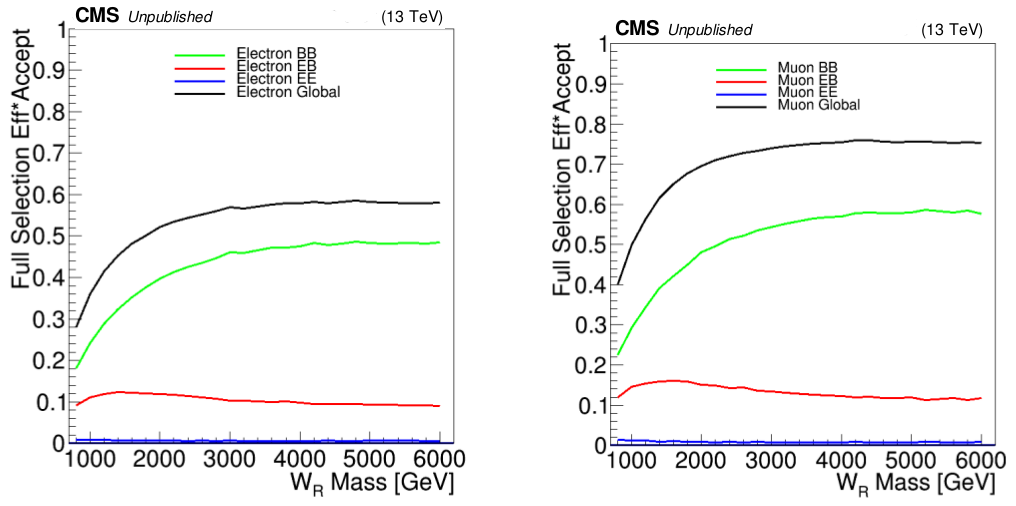
\includegraphics[width=1.0\textwidth]{figures/wrRecoSelectionEfficiency.png}
	\caption{The efficiency that $\WR \rightarrow \ell\nul \rightarrow \ell\ell jj$ events are selected using 
	the trigger and full offline selection in the ee ($\mu\mu$) -channel on the left (right).  Different curves represent 
events where both leptons were in the barrel $\eta$ region (BB), one was in the endcap (EB), or both were in the endcap (EE).}
	\label{fig:wrRecoSelectionEff}
\end{figure}

LRS models predicted a signal from a \WR boson and heavy neutrino \nul manifested as an excess of events relative 
to expected backgrounds in distributions of several lepton and jet kinematic variables, like $\pt$ and multi-particle 
invariant masses.  Models differed in the shapes and magnitudes of predicted excesses, but all agreed on one point: 
a \WR boson existed, and evidence of it appeared as a peak in the \Mlljj distribution, whose peak position was consistent 
with the predicted \mWR.  To look for evidence in support of LRS models without being sensitive to nuances of different 
models, the \Mlljj mass was used as the search variable of merit.  Shown in Figure \ref{fig:mlljjVariableOfMerit} was 
proof of this variable's efficacy: a simulated \WR signal with $\mWR = 1.0, \mnul = 0.5 \TeV$ appeared as a sharp peak 
in the \Mlljj distribution centered near $\Mlljj = 1.0 \TeV$ that was clearly differentiated from expected ST backgrounds.

\begin{figure}[h]
	\centering
	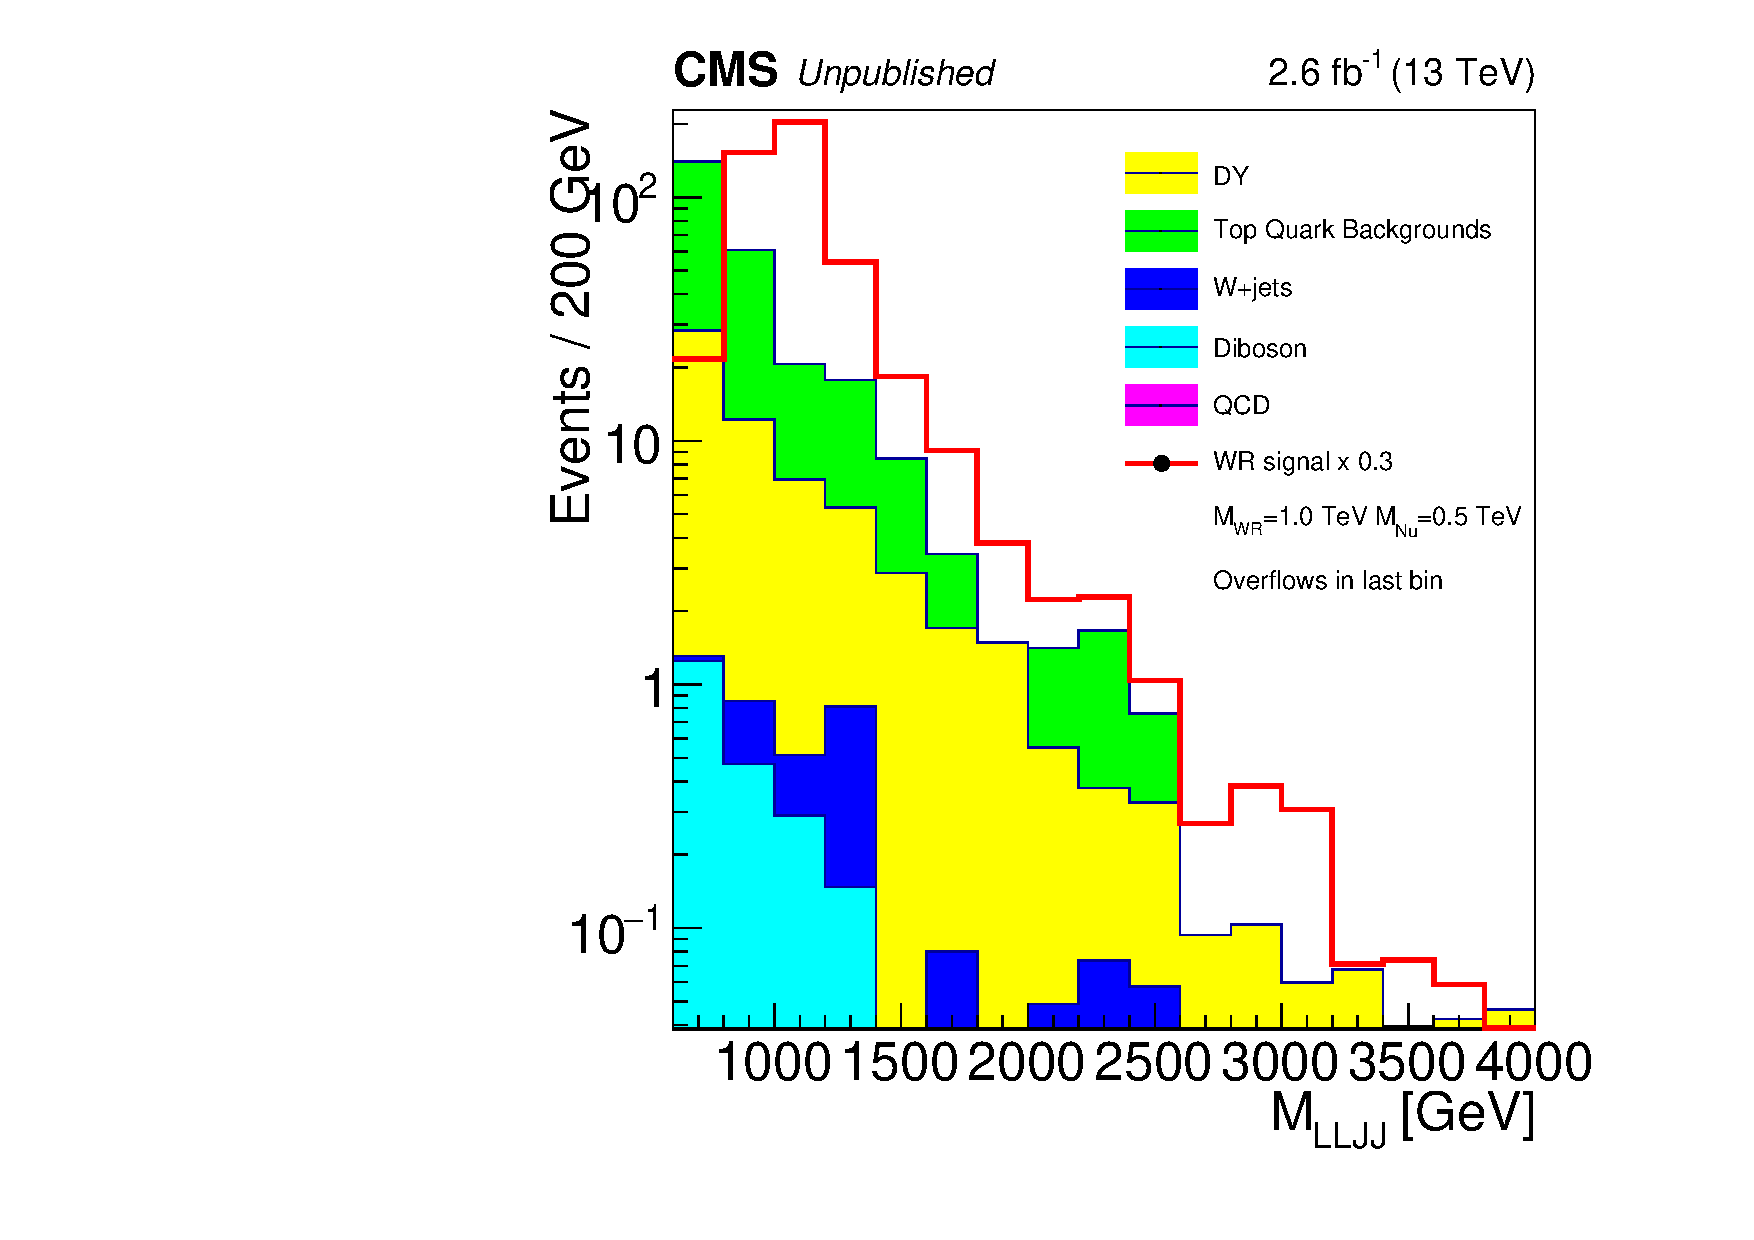
\includegraphics[width=0.7\textwidth]{figures/useOfLLJJMassAsFigureOfMerit.pdf}
	\caption{The $\Mlljj$ distribution from simulations of expected ST backgrounds and \WR signal in the ee -channel.  
		The normalization of the \WR signal distribution is scaled down by 70\% only to better visualize the difference 
	between \WR signal and expected backgrounds.}
	\label{fig:mlljjVariableOfMerit}
\end{figure}



%%%%%%%%%%%%%%%%%%%%%%%%%%%%%%%%%%%%%%%%%%%%%%%%%%%%%%%%%%%%%%%%%%%%%%%%%%%%%%%%
